\documentclass[sigconf]{acmart}

\usepackage{booktabs} % For formal tables
\usepackage{amsmath}
\usepackage{tipa}
\usepackage{subcaption}
\usepackage{graphicx}
\usepackage{hyperref}
\usepackage{parskip}
\usepackage{minted}
\usepackage{xcolor}
% Copyright
\setcopyright{none}
%\setcopyright{acmcopyright}
%\setcopyright{acmlicensed}
%\setcopyright{rightsretained}
%\setcopyright{usgov}
%\setcopyright{usgovmixed}
%\setcopyright{cagov}
%\setcopyright{cagovmixed}


% DOI
\acmDOI{ }

% ISBN
\acmISBN{ }

%Conference
\acmConference[DTU]{DTU conference}{\today}{Kgs Lyngby, Denmark} 
\acmYear{1997}
\copyrightyear{2017}


\acmArticle{1}
\acmPrice{3.50}

% These commands are optional
%\acmBooktitle{Transactions of the ACM Woodstock conference}
%\editor{Roar Nind Steffensen}


\begin{document}
\title{Midterm 2 - Operating Systems}
%\titlenote{Produces the permission block, and copyright information}
\subtitle{Roar Nind Steffensen (s144107)}
%\subtitlenote{The full version of the author's guide is available as
%  \texttt{acmart.pdf} document}


%\author{Ben Trovato}
%\authornote{Dr.~Trovato insisted his name be first.}
%\orcid{1234-5678-9012}
%\affiliation{%
%  \institution{Institute for Clarity in Documentation}
%  \streetaddress{P.O. Box 1212}
%  \city{Dublin} 
%  \state{Ohio} 
%  \postcode{43017-6221}
%}
%\email{trovato@corporation.com}

% The default list of authors is too long for headers.
\renewcommand{\shortauthors}{B. Trovato et al.}


%\begin{abstract}
%This paper provides a sample of a \LaTeX\ document which conforms, somewhat loosely, to the formatting guidelines for ACM SIG Proceedings.\footnote{This is an abstract footnote}
%\end{abstract}

%
% The code below should be generated by the tool at
% http://dl.acm.org/ccs.cfm
% Please copy and paste the code instead of the example below. 
%
%\begin{CCSXML}
%<ccs2012>
% <concept>
%  <concept_id>10010520.10010553.10010562</concept_id>
%  <concept_desc>Computer systems organization~Embedded systems</concept_desc>
%  <concept_significance>500</concept_significance>
% </concept>
% <concept>
%  <concept_id>10010520.10010575.10010755</concept_id>
%  <concept_desc>Computer systems organization~Redundancy</concept_desc>
%  <concept_significance>300</concept_significance>
% </concept>
% <concept>
%  <concept_id>10010520.10010553.10010554</concept_id>
%  <concept_desc>Computer systems organization~Robotics</concept_desc>
%  <concept_significance>100</concept_significance>
% </concept>
% <concept>
%  <concept_id>10003033.10003083.10003095</concept_id>
%  <concept_desc>Networks~Network reliability</concept_desc>
%  <concept_significance>100</concept_significance>
% </concept>
%</ccs2012>  
%\end{CCSXML}

%\ccsdesc[500]{Computer systems organization~Embedded systems}
%\ccsdesc[300]{Computer systems organization~Redundancy}
%\ccsdesc{Computer systems organization~Robotics}
%\ccsdesc[100]{Networks~Network reliability}


\keywords{Processes, Threads, Schedulers, Fairness}

\maketitle


\section{Operating system organization}
\subsection*{Question 1.1}
%Explain, in your own words, the differences and similarities between an operating system with a monolithic kernel and a exo-kernel based operating system.

For an operating system to be exo-kernel (according to the \texttt{Modern Operating System} \cite{tanembaum}, section 1.7.6), the users must have direct access to hardware. This approach is often used for e.g. virtual machines, where the operating system is simulating several systems. The exo-kernel's main job is, to restrict each virtual machine to their respective resources, thereby hinder the virtual machines to access each others resources such as memory. 

Monolithic is the most common (\texttt{Moden Operating Systems} section 1.7.1) and undefined operating system structure. The operating system is often defined as a single single program running in kernel mode. All procedures can call each other, but can easily become chaotic / entangled. For that reason, the operating system may be divided up into layers, creating levels of abstraction to organize the control flow.

For monolithic operating systems, the user/programs do not necessary have access to the hardware directly, as in an exo-kernel operating system. Otherwise both operating systems, in general needs a security manager, scheduler, memory manager, and Input/Output manager, and operate from user-mode to kernel-mode through system calls and traps.

\section{Scheduling and synchronization}
\subsection*{Question 2.1}
%Race conditions can occur with preemptive scheduling. Explain why. Show with an example, of your own, how such race conditions can be eliminated.

Race conditions occurs, when the intended result of a (or several) program(s) is sensitive to the order of executions among the threads. These unwanted behaviors are often linked with memory access, as when two threads access the same address in the address space, and both threads update the value. If both threads read the initial value, say 50, and both threads intend to increment the value by 5, then the first thread will write 55 to the address, as expected, but the second thread will also write 55 to the address, overwriting the first threads change. 

These problems occur once concurrent executions are introduced to the systems, and must be handled with care. To prevent such race conditions, mutual exclusion must be implemented so that the threads can execute their operations which might otherwise result in race conditions independently. These groups of operations are also known as critical sections. When several threads try to access a shared resource, and race conditions may occur, all the threads may have critical sections which must handled with mutual exclusion, these sets of critical sections are known as critical regions.

A way to implement mutual exclusion, is with a "Test-and-Set-Lock" operation (TSL) which uses hardware support as mentioned in \texttt{Modern Operating Systems} section 2.3.3. Any software implementation of mutual exclusion is itself in risk of race conditions, which is why hardware support is needed. The TSL operation reads the value at an address, sets the value to a specific value and returns the previous value. The value operated upon by such an operation is often referred to, as a lock (with a key), and the read/write procedure is executed in the same use of the bus, thereby denying preemptive operations to alter the value at the specific address between reading and writing. The TSL operation is then called through a system call, before a thread enters its critical section, until access is granted (the key is received), making it certain, that no other TSL calls on that address will grant access, until the thread leaves the critical section by writing the key back to the address. 

\subsection*{Question 2.2}
%During their lifetime, threads can be in different states. What states? Form a statemachine with the states and all possible transitions. Explain with your own words, what each state and transition mean.

According to \texttt{Modern Operating Systems} section 2.2.1-2, threads are seen as "mini processors" (though sharing resources), the threads contain the same states as a processor: \textit{ready}, \textit{blocked} and \textit{ready}. But depending on how you evaluate a thread when it is killed, we also have the state \textit{terminated}. The states, and the transitions between them, are outlined in the state machine in figure \ref{fig:threadstates}.

\begin{figure}[H]
    \centering
    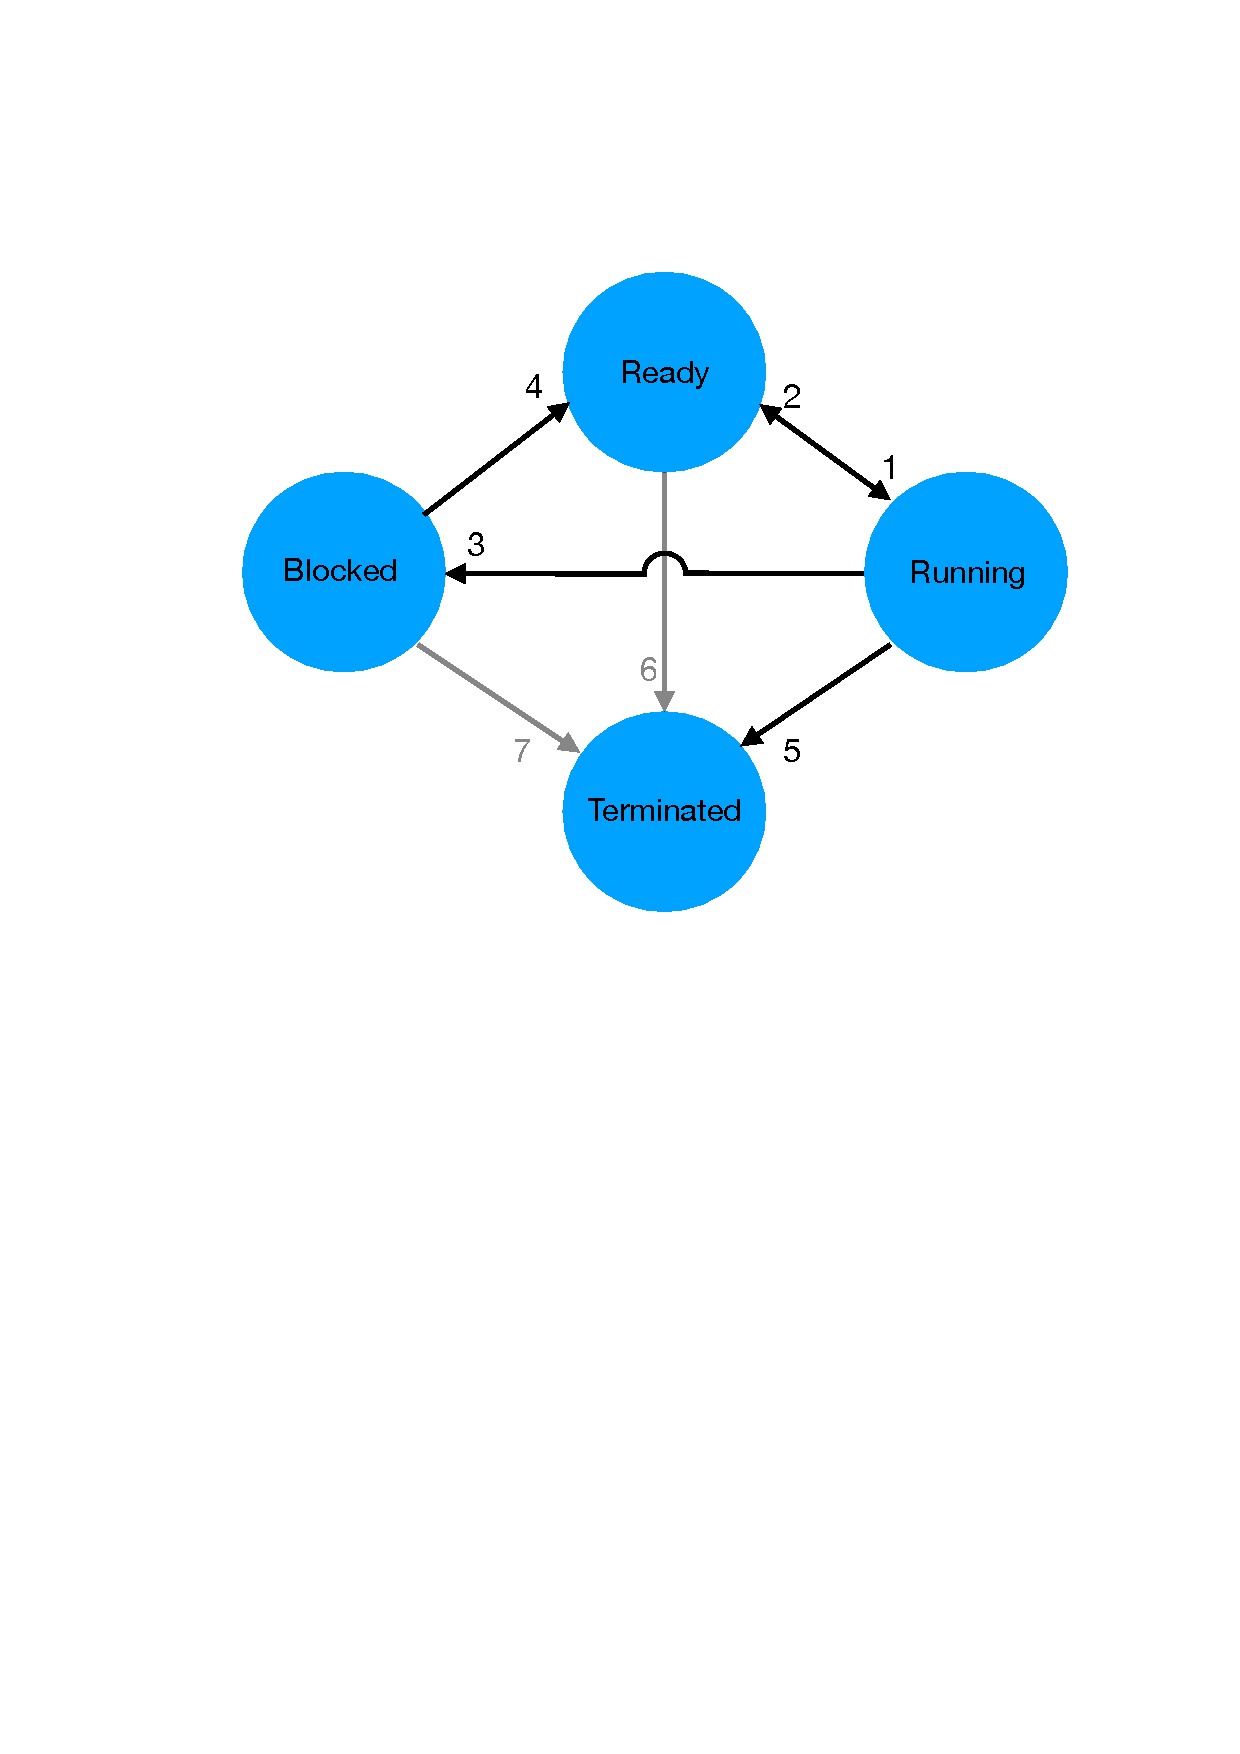
\includegraphics[width=0.9\linewidth]{ThreadStates.pdf}
    \caption{States and transitions of a thread.}
    \label{fig:threadstates}
\end{figure}

The states are evaluated as:

\textbf{Ready:} Waiting to get CPU time from the scheduler.\\
\textbf{Blocked:} Not given time by the scheduler. Possibly while requesting input from an input device.\\
\textbf{Running:} Given time by the scheduler and executing operations.\\
\textbf{Terminated:} Removed and resources are freed.\\

The transitions are evaluated as:
\begin{enumerate}
    \item The thread has been given time by the scheduler and can begin to execute.
    \item The thread is paused (placed in the scheduler queue) and waits until execution can proceed.
    \item When blocked, a thread is set aside until unblocked by a dispatching thread.
    \item A thread going from \textit{blocked} state to \textit{ready} state is woken up by the dispatcher, and is now waiting to execute in \textit{running} state.
    \item When a thread either crashes or finishes execution it will terminate.
    \item A blocked thread being terminated directly. If the thread was blocked until an input was received, but the input device was removed, the thread may be terminated depending on implementation.
    \item Like transition 6, a thread may be terminated while waiting to proceed execution, e.g. if the process containing the thread is killed.
\end{enumerate}

For transitions 6 and 7, it would often be recommended to throw an interrupt, waking the thread up, and ensuring that it is terminated in a safe place, meaning that transitions 6 and 7 would be removed, as it would go through the \textit{ready} and \textit{running} state. If threads are kept in a static array, and reused between processes, the \textit{terminate} state just act as a special \textit{blocked} state. 

Threads are quite analogous to good workers, as they either work, wait to work, are told not to work until further notice or are dead.

\subsection*{Question 2.3}
%What data structures are needed to implement a scheduler?
The data structures to implement a scheduler depends on what algorithm the scheduler is intended to use. The scheduler must have access to the processes and threads to get information on what jobs should be scheduled. Some of the algorithms from \texttt{Modern Operating Systems} are outlined.

If a simple \textit{round robin} algorithm is implemented, the scheduler only needs to scan the threads (or processes with child threads) to find the next ready thread. Either the threads can run to completion or be given a time interval, also known as a quantum, where it can execute, until the next thread is scheduled in the same manner. This scheduling algorithm effectively assumes that all jobs are equally prioritized, although this may not be the case. A prioritized version, with access to different priorities of the jobs, may use \textit{round robin} between the most prioritized jobs.

Alternatively the used algorithm could be \textit{First-Come, First-Served} as in a FIFO queue where processes are scheduled in order by the request. This would need a list of processors e.g. by a linked list.

If the execution times for the processors are known beforehand, a \textit{Shortest Job First} algorithm can be used. This would need a list of processors with their respective times, optimally sorted in non-descending order by execution times. The first element will be the process with the shortest job and will be given highest priority. A preemptive version of this algorithm exists, where the threads may be stopped mid-execution and the process with the shortest time remaining will be given priority.

Many such algorithms exist, but the majority uses a queue of processors(or threads) together with some information about them to determine the next job to schedule, leading to data structures such as a list or table of pointers or id's to the processors and the required information. If efficient sorting is prioritized, a data structure such as a max-heap would make inserting and extracting elements run in \texttt{O}($\log$(N)) time.

\subsection*{Question 2.4}
%What does it mean that a scheduler is fair? How can you ensure fairness in a scheduler?

Fairness can be divided up into weak fairness and strong fairness, as mentioned in the course notes for the Concurrent Programming course, section 4.6 \cite{coursenotes}. 

Weak fairness ensures that if a process is continuously ready to execute, then it will execute at some point. 

Strong fairness ensures that if a process has infinitely many possibilities to execute, then it will execute at some point. 

For computer systems, weak fairness is often the used fairness implementation. This is seen in figure \ref{fig:threadstates} as only threads in the \textit{ready} state can transition to the \textit{running} state. 

For a system to be strongly fair, even if a process switches between being ready and not ready to proceed, it would then be certain that the process proceeds at some point. Corresponding to a process appearing and disappearing from the scheduler queue indefinitely without being chosen by the scheduler. Since information on the complete history of the process may be needed, this would be exhaustive. This behavior is often refrained from in such systems meaning that often only weak fairness is necessary.

In order to make the algorithms mentioned above fair, some of them needs to be altered slightly. The \textit{round robin} and the \textit{First-Come, First-Served} are inherently fair, since no priority is given. The prioritized version needs to give higher priority to processors which have waited, resulting in them eventually being chosen. Likewise for the \textit{shortest job first} algorithms, the processors which have waited longest needs to get priority, here by having their execution times lowered (making it a pseudo execution time). 

This way prioritizing algorithm may eventually pick a waiting process, independent of its first priority, ensuring that at the algorithm implements weak fairness.

\bibliographystyle{ACM-Reference-Format}
\bibliography{bibliography} 

\end{document}
